\documentclass [xcolor=svgnames, notes] {beamer}
% \usepackage{enumitem}
\usepackage[utf8]{vietnam}
\usepackage{xcolor}
\usepackage{booktabs, comment, multirow}
\usepackage{pgfpages}
\usepackage{csquotes}
\usepackage{amsmath, amssymb, amsthm}
\usepackage{bm}
\usepackage{tikz}
\usetheme{Madrid}

\usepackage[linesnumbered,ruled,vlined]{algorithm2e}

\usepackage[style=numeric, sorting=none]{biblatex}
\AtBeginBibliography{\tiny}  % Áp dụng \small cho phần bibliography
\addbibresource{References.bib}
\usepackage{longtable}

% COLORS
\definecolor{mqred}{RGB}{166, 25, 46}
\definecolor{mqdeepred}{RGB}{118, 35, 47}
\definecolor{mqgray}{RGB}{55, 58, 54}
\definecolor{mqlightgray}{RGB}{237, 235, 229}
\definecolor{mqmagenta}{RGB}{198, 0, 126}
\usecolortheme[named=mqred]{structure}
\setbeamercolor{title in head/foot}{bg=mqlightgray, fg=mqgray}
\setbeamercolor{author in head/foot}{bg=mqdeepred}
\setbeamercolor{page number in head/foot}{bg=mqdeepred, fg=mqlightgray}

% FOOTNOTE ARRANGEMENTS

\makeatletter
\setbeamertemplate{footline}{
  \leavevmode%
  \hbox{%
  \begin{beamercolorbox}[wd=.4\paperwidth,ht=2.25ex,dp=1ex,center]{author in head/foot}%
    \usebeamerfont{author in head/foot}\insertshortauthor\expandafter\ifblank\expandafter{\beamer@shortinstitute}{}{~~(\insertshortinstitute)}
  \end{beamercolorbox}%
  \begin{beamercolorbox}[wd=.3\paperwidth,ht=2.25ex,dp=1ex,center]{title in head/foot}%
    \usebeamerfont{title in head/foot}\insertshorttitle
  \end{beamercolorbox}%
  \begin{beamercolorbox}[wd=.2\paperwidth,ht=2.25ex,dp=1ex,center]{date in head/foot}%
    \usebeamerfont{date in head/foot}\insertshortdate
  \end{beamercolorbox}%
  \begin{beamercolorbox}[wd=.1\paperwidth,ht=2.25ex,dp=1ex,center]{page number in head/foot}%
    \usebeamerfont{page number in head/foot}\insertframenumber{} / \inserttotalframenumber
  \end{beamercolorbox}}%
  \vskip0pt%
}
\makeatother
\beamertemplatenavigationsymbolsempty
\setbeamerfont{author}{size=\small}
\setbeamerfont{footnote}{size=\tiny}

% Trích dẫn dạng chú thích chân trang: Tác giả (năm): "Tên bài".
\newcommand{\refnote}[1]{\footnote{\citeauthor{#1} (\citeyear{#1}): ``\citefield{#1}{title}''.}}
\newcommand{\R}{\mathbb{R}}
\newcommand{\one}{\mathbf{1}}

% TITLE, AUTHORS, INSTITUTE, DATE

\title[Đồ án 1]{\textbf{Kết hợp học quan hệ động giữa các biến và dự báo theo đoạn dựa trên thành phần cơ sở cho chuỗi thời gian đa biến}}
\author[Sinh viên thực hiện: Nguyễn Hải Long]{
\begin{tabular}{ll}
    \textbf{Giảng viên hướng dẫn:} & \color{mqred}{\textbf{PGS. TS. Nguyễn Thị Ngọc Anh}} \\
    \textbf{Sinh viên thực hiện:}  & \color{mqred}{\textbf{Nguyễn Hải Long}} \\
    \textbf{Mã số sinh viên:}      & \color{mqred}{\textbf{20237355}}
\end{tabular}
}
% \institute[]{Đại học Bách khoa Hà Nội}
% LOGO
% \titlegraphic{
\includegraphics[height=2cm]{logo/hust.png}   \hspace{0.5cm}
%               
\includegraphics[height=2cm]{logo/fami.png}} % Change the logo path as needed

\date[Tháng 10, 2026]{Hà Nội, 10/2026}

\begin{document}
\begin{frame}
    \centering
    
\includegraphics[height=1.5cm]{logo/hust.png}
    
\includegraphics[height=1.5cm]{logo/fami_1.png}
    \titlepage
\end{frame}
\begin{frame}{Nội dung chính}
    \tableofcontents
\end{frame}
\AtBeginSection[]{
\begin{frame}{Mục lục}
    \tableofcontents[currentsection]
\end{frame}
}

%=====================================================================
\section{Tổng quan vấn đề nghiên cứu và mục đích nghiên cứu}
\subsection{Tổng quan vấn đề nghiên cứu}

\begin{frame}{Bài toán dự báo dài hạn chuỗi thời gian đa biến}
\begin{itemize}
    \item \textbf{Bài toán:} từ $L$ bước quá khứ của $C$ biến, dự báo đồng thời $S$ bước tương lai của cả $C$ biến
          (năng lượng, thời tiết, giao thông\dots).

    \vspace{0.15cm}
    \item \textbf{Xu hướng hiện nay:} dùng cửa sổ quá khứ rất dài ($L = 720$) để nắm phụ thuộc dài hạn, kéo theo số
          tham số và khối lượng tính toán tăng mạnh\refnote{Huang2025TimeBase}.

    \vspace{0.15cm}
    \item \textbf{Hai yêu cầu cần đáp ứng cùng lúc:}
    \begin{itemize}
        \item \emph{Nhẹ và nhanh}, để triển khai được trên thiết bị hạn chế tài nguyên.
        \item \emph{Khai thác quan hệ giữa các biến}, vì các biến trong hệ thống thực ảnh hưởng lẫn nhau.
    \end{itemize}
\end{itemize}
\end{frame}

\begin{frame}{Đặc điểm 1: Tính lặp lại}
\begin{itemize}
    \item \textbf{Tương đồng theo chu kỳ:} các đoạn dài một chu kỳ (ví dụ mỗi ngày) có hình dạng rất giống nhau, với hệ số
          tương quan Pearson giữa các đoạn cao\refnote{Huang2025TimeBase}.

    \vspace{0.15cm}
    \item \textbf{Hệ quả:} không nhất thiết phải mô hình hóa từng điểm thời gian. TimeBase chỉ dùng
          \textbf{0.39K tham số}, ít hơn DLinear hơn $2.6\times10^{3}$ lần về tham số và 120 lần về MACs, mà vẫn đạt độ chính
          xác cạnh tranh.
\end{itemize}

\vspace{0.2cm}
\begin{block}{}
\centering Dự báo trên \textbf{một vài ``đoạn đại diện''} thay vì trên $L$ điểm thời gian.
\end{block}
\end{frame}

\begin{frame}{Đặc điểm 2: Phụ thuộc chéo giữa các biến}
\begin{itemize}
    \item Các phương pháp chia làm hai nhóm theo cách xử lý biến\refnote{Han2024Capacity}:
    \begin{itemize}
        \item \textbf{Độc lập biến (CI)} (PatchTST, DLinear, TimeBase): mỗi biến dự báo riêng, bỏ qua các quan hệ hiệp
              biến quan trọng.
        \item \textbf{Phụ thuộc biến (CD)} (iTransformer, DyTimeNet): học mọi phụ thuộc mà không phân biệt, đưa thêm nhiễu
              và giảm khả năng khái quát\refnote{Hu2025TimeFilter}.
    \end{itemize}

    \vspace{0.15cm}
    \item \textbf{Mức phụ thuộc khác nhau theo miền dữ liệu:} biến khí hậu có ràng buộc vật lý tự nhiên với nhau, còn mức
          tiêu thụ điện của từng hộ gần như độc lập.

    \vspace{0.15cm}
    \item \textbf{Phụ thuộc chéo thay đổi theo thời gian và thưa:} DyTimeNet dùng chiến lược thưa \emph{DropFusion} để
          giảm thông tin dư thừa khi học quan hệ liên biến\refnote{Chen2026DyTimeNet}.
\end{itemize}
\end{frame}

\begin{frame}{Khoảng trống nghiên cứu}
\small
\begin{center}
\resizebox{\textwidth}{!}{%
\begin{tabular}{@{}llcc@{}}
\toprule
Nhóm mô hình & Ví dụ & Rất nhẹ & Học quan hệ liên biến\\
\midrule
Tuyến tính theo đoạn / tần số, CI & TimeBase, SparseTSF, FITS & \textcolor{ForestGreen}{\checkmark} & \textcolor{mqred}{$\times$}\\
Transformer & PatchTST, iTransformer & \textcolor{mqred}{$\times$} & một phần\\
Đồ thị, lọc phụ thuộc theo patch & TimeFilter & \textcolor{mqred}{$\times$} & \textcolor{ForestGreen}{\checkmark}\\
MLP trộn biến trên chuỗi gốc (chi phí theo $L$, $S$) & DyTimeNet & \textcolor{mqred}{$\times$} & \textcolor{ForestGreen}{\checkmark}\\
\bottomrule
\end{tabular}}
\end{center}

\begin{itemize}
    \item \refnote{Huang2025TimeBase}TimeBase giả định các biến \emph{đồng nhất} nên dùng chiến lược độc lập biến.
    \item \refnote{Hu2025TimeFilter}TimeFilter dựng đồ thị trên $n = C\times N$ nút (biến, patch); ma trận khoảng cách có kích thước
          $n\times n$.
\end{itemize}

\begin{alertblock}{Khoảng trống}
Chưa có mô hình vừa giữ chi phí siêu nhẹ của dự báo theo đoạn, vừa học được phụ thuộc chéo giữa các biến.
\end{alertblock}
\end{frame}

\subsection{Mục đích nghiên cứu}

\begin{frame}{Mục đích nghiên cứu}
Đề xuất mô hình \textbf{DyBAS-Net} (\textbf{Dy}namic cross-variable dependency on \textbf{BAS}is components), kết hợp hai
hướng tiếp cận:

\vspace{0.15cm}
\begin{itemize}
    \item \textbf{Dự báo theo đoạn:} phân đoạn theo chu kỳ, trích xuất $R$ thành phần cơ sở và dự báo theo
          đoạn, kế thừa từ TimeBase\refnote{Huang2025TimeBase}.

    \item \textbf{Học phụ thuộc chéo trong không gian cơ sở:} đưa CrossVBlock với chiến lược DropFusion và IntraVBlock của
          DyTimeNet\refnote{Chen2026DyTimeNet} vào xử lý $P\cdot R$ hệ số cơ sở của mỗi biến, thay vì $L$ điểm thời gian.

    \item \textbf{Hiệu chỉnh có kiểm soát:} nhánh trộn biến chỉ cộng một lượng hiệu chỉnh vào các thành phần cơ sở, được
          khởi tạo bằng 0.

    \item \textbf{Đánh giá toàn diện:} 5 bộ dữ liệu, so sánh với 11 mô hình về độ chính xác và chi phí tính toán trên
          \emph{cùng một thiết bị}.
\end{itemize}
\end{frame}

%=====================================================================
\section{Phương pháp luận}
\subsection{Mô hình hóa toán học}

\begin{frame}{Input}
    \small
    \textbf{Dữ liệu tập train $\mathcal{X}_{train} \in \mathbb{R}^{L \times C}$:} Chuỗi lịch sử độ dài $L$ của $C$ biến
    $X^{(i)}$ với $i = \overline{1, C}$.

    \begin{columns}[c]
        \begin{column}{0.52\textwidth}
            \[
            \mathcal{X}_{train} =
            \begin{bmatrix}
            x_1^{(1)} & x_1^{(2)} & \dots & x_1^{(C)} \\
            x_2^{(1)} & x_2^{(2)} & \dots & x_2^{(C)} \\
            \vdots & \vdots & \ddots & \vdots \\
            x_L^{(1)} & x_L^{(2)} & \dots & x_L^{(C)}
            \end{bmatrix}
            \]
        \end{column}
        \begin{column}{0.45\textwidth}
            \textbf{Định nghĩa thành phần:}
            \begin{itemize}
                \setlength{\itemsep}{2pt}
                \item $x_t^{(i)}$: Giá trị của biến $X^{(i)}$ tại thời điểm $t$.
                \item $i = \overline{1, C}$: Chỉ số biến.
                \item $t = \overline{1, L}$: Chỉ số mốc thời gian.
            \end{itemize}
        \end{column}
    \end{columns}

    \vspace{0.1cm}
    \textbf{Dữ liệu tập test $\mathcal{X}_{test} \in \mathbb{R}^{S \times C}$:} Giá trị thực tế trong $S$ bước tiếp theo:
    \[
    \mathcal{X}_{test} =
    \begin{bmatrix}
    x_{L+1}^{(1)} & x_{L+1}^{(2)} & \dots & x_{L+1}^{(C)} \\
    \vdots & \vdots & \ddots & \vdots \\
    x_{L+S}^{(1)} & x_{L+S}^{(2)} & \dots & x_{L+S}^{(C)}
    \end{bmatrix}
    \]
\end{frame}

\begin{frame}{Output và Hàm mục tiêu}
    \begin{itemize}
        \item \textbf{Ma trận kết quả dự báo ($\hat{\mathcal{X}} \in \mathbb{R}^{S \times C}$):} được ước lượng đồng thời
              bởi mô hình $\mathcal{F}$ (\textbf{DyBAS-Net}):
        $$\hat{\mathcal{X}} = \mathcal{F}(\mathcal{X}_{train})$$

        \item \textbf{Sai số dự báo (MSE):}
        $$ \mathcal{L}_{MSE} = \frac{1}{S \times C} \sum_{t=1}^{S} \sum_{i=1}^{C} \left( x_{L+t}^{(i)} - \hat{x}_{L+t}^{(i)} \right)^2$$

        \item \textbf{Hàm mục tiêu khi huấn luyện:} thêm ràng buộc trực giao trên các thành phần cơ sở:
        $$\mathcal{L} = \mathcal{L}_{MSE} + \lambda_{orth}\,\mathcal{L}_{orth}, \qquad \lambda_{orth}\ge 0$$
    \end{itemize}
\end{frame}

\begin{frame}{Các kích thước sử dụng trong mô hình}
\begin{center}
\resizebox{\textwidth}{!}{%
\begin{tabular}{@{}cll@{}}
\toprule
Ký hiệu & Ý nghĩa & ETTh1 ($L=720$, $S=96$)\\
\midrule
$P$ & Độ dài một đoạn (chu kỳ) & $24$ (một ngày) \\
$N=\lceil L/P\rceil$ & Số đoạn quá khứ & $30$ ngày \\
$N'=\lceil S/P\rceil$ & Số đoạn tương lai & $4$ ngày \\
$R \ll N$ & Số thành phần cơ sở & $6$ \\
$D$ & Số chiều ẩn của nhánh trộn biến & $64$ \\
$C'=\lfloor 0.75\,C\rfloor$ & Số chiều nút thắt của CrossVBlock & $5$ \\
$D_{ff}=2D$ & Số chiều ẩn của FFN trong IntraVBlock & $128$ \\
\bottomrule
\end{tabular}}
\end{center}
\end{frame}

\begin{frame}{Kiến trúc cơ bản của các mô hình dự báo CTG}
\centering
    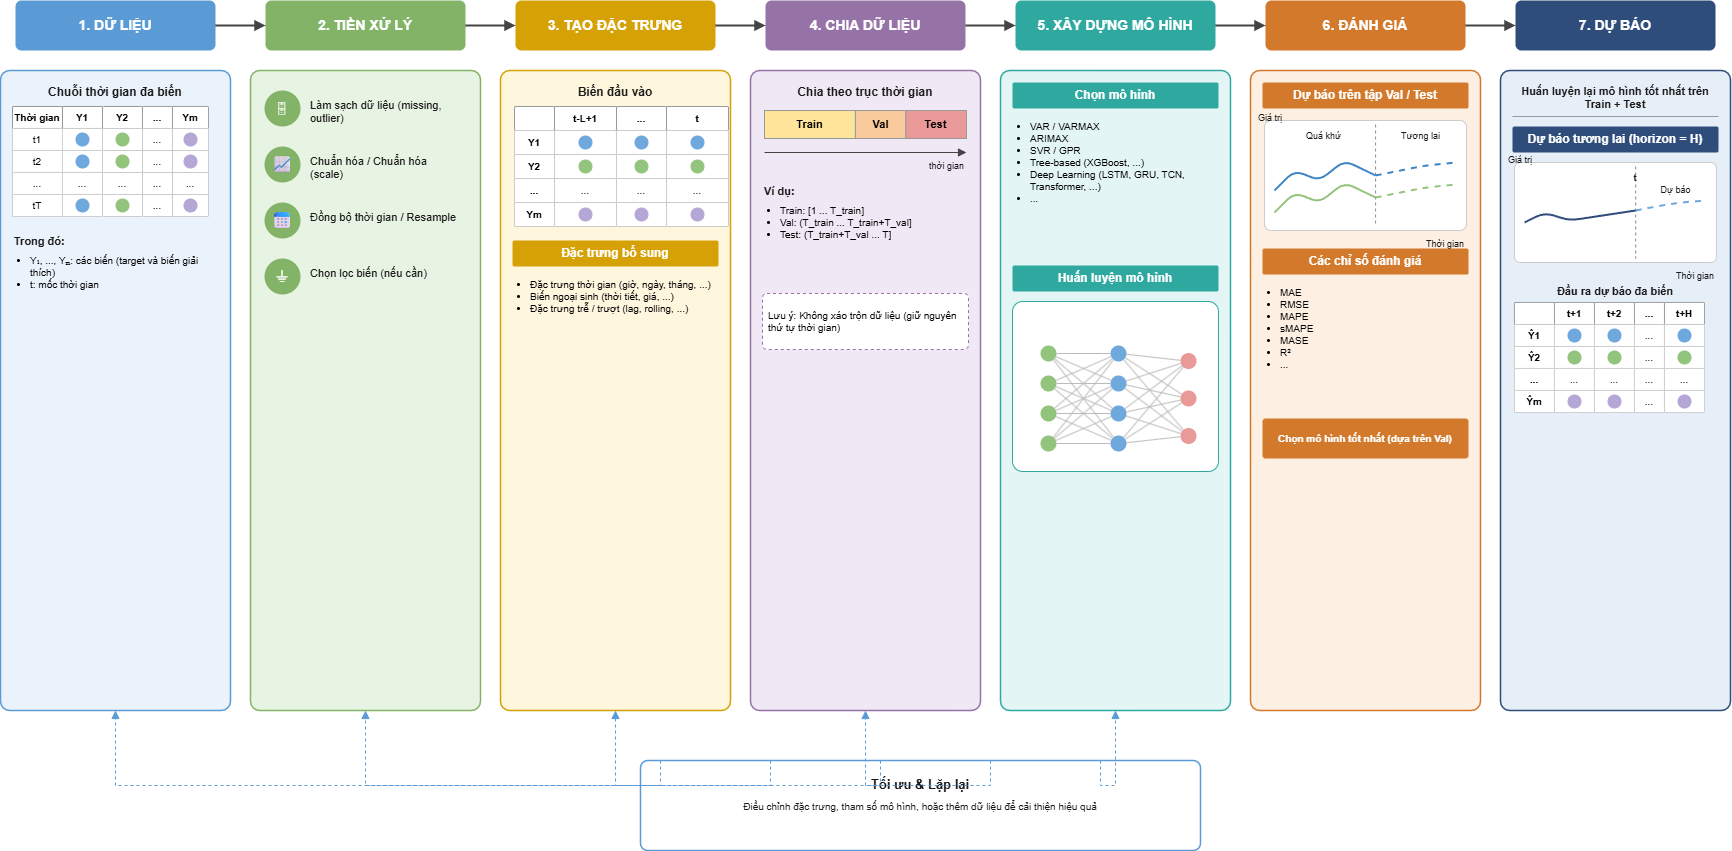
\includegraphics[width=1\linewidth]{pipeline_tong_quat.png}
\end{frame}

\subsection{Xây dựng mô hình}

\begin{frame}{Tổng quan các bước của DyBAS-Net}
\begin{enumerate}
    \item \textbf{Phân đoạn theo chu kỳ:} cắt chuỗi dài $L$ thành $N$ đoạn dài $P$.
    \item \textbf{Chuẩn hóa theo pha:} trừ trung bình của từng pha trong chu kỳ.
    \item \textbf{Trích xuất cơ sở:} nén $N$ đoạn thành $R$ thành phần cơ sở $\mathbf{E}^{(i)}$.
    \item \textbf{Mã hóa hệ số cơ sở} của mỗi biến thành vector $D$ chiều.
    \item \textbf{CrossVBlock + DropFusion:} trộn thông tin giữa các biến.
    \item \textbf{IntraVBlock:} biến đổi phi tuyến trong từng biến.
    \item \textbf{Chiếu ngược:} sinh lượng hiệu chỉnh $\Delta\mathbf{E}^{(i)}$, cộng vào cơ sở.
    \item \textbf{Dự báo theo đoạn và khôi phục:} sinh $N'$ đoạn tương lai, cộng lại trung bình theo pha.
\end{enumerate}

\end{frame}

\begin{frame}{1. Phân đoạn theo chu kỳ}
\small
Chuỗi của biến $i$, $\mathbf{x}^{(i)} = (x^{(i)}_1,\dots,x^{(i)}_L)$, được xếp thành \textbf{ma trận đoạn}
$\mathbf{X}^{(i)}\in\R^{P\times N}$, mỗi cột là một đoạn dài $P$:
\[
\mathbf{X}^{(i)} =
\begin{bmatrix}
x^{(i)}_1 & x^{(i)}_{P+1} & \dots & x^{(i)}_{(N-1)P+1}\\
x^{(i)}_2 & x^{(i)}_{P+2} & \dots & x^{(i)}_{(N-1)P+2}\\
\vdots & \vdots & \ddots & \vdots\\
x^{(i)}_P & x^{(i)}_{2P} & \dots & x^{(i)}_{NP}
\end{bmatrix},
\qquad \big[\mathbf{X}^{(i)}\big]_{p,n} = x^{(i)}_{(n-1)P+p}
\]
\begin{itemize}
    \item \textbf{Cột} $n$: đoạn thứ $n$ (ví dụ ngày thứ $n$). \textbf{Hàng} $p$: cùng một pha (ví dụ cùng một giờ) qua $N$
          chu kỳ.
    \item Ví dụ ETTh1: $L=720$, $P=24$ $\Rightarrow$ $N=30$ cột, mỗi cột là một ngày.
    \item Nếu $L$ không chia hết cho $P$, chuỗi được đệm thêm ở đầu cho đủ $N\cdot P$ điểm.
\end{itemize}
\end{frame}

\begin{frame}{2. Chuẩn hóa theo pha}
\begin{itemize}
    \item \textbf{Trung bình theo pha:} trung bình của từng hàng (từng pha) qua $N$ đoạn:
    $$\mu^{(i)}_p = \frac{1}{N}\sum_{n=1}^{N}\big[\mathbf{X}^{(i)}\big]_{p,n},
      \qquad \bm{\mu}^{(i)} = (\mu^{(i)}_1,\dots,\mu^{(i)}_P)^{\top}\in\R^{P}$$

    \item \textbf{Trừ trung bình:}
    $$\big[\tilde{\mathbf{X}}^{(i)}\big]_{p,n} = \big[\mathbf{X}^{(i)}\big]_{p,n} - \mu^{(i)}_p
      \qquad (\text{trừ } \mu^{(i)}_p \text{ cho mọi phần tử của hàng } p)$$

    \item \textbf{Ý nghĩa:} $\bm{\mu}^{(i)}$ là ``đoạn trung bình'' của biến $i$ (ví dụ ban ngày phụ tải cao hơn ban đêm).
          Các bước sau chỉ học phần dao động quanh nó.
\end{itemize}
\end{frame}

\begin{frame}{3. Trích xuất thành phần cơ sở (Basis Extraction)}
\begin{itemize}
    \item Ánh xạ tuyến tính \textbf{dùng chung cho mọi biến} nén $N$ đoạn thành $R$ thành phần cơ sở
          ($\mathbf{W}_B\in\R^{N\times R}$, $\mathbf{b}_B\in\R^{R}$ học được):
    $$\mathbf{E}^{(i)} = \tilde{\mathbf{X}}^{(i)}\,\mathbf{W}_B + \mathbf{b}_B \quad\in\R^{P\times R}
      \qquad (\mathbf{b}_B \text{ cộng vào mọi hàng})$$

    \item \textbf{Cột thứ $r$ của $\mathbf{E}^{(i)}$} là tổ hợp tuyến tính của $N$ đoạn quá khứ
          $\tilde{\mathbf{x}}^{(i)}_n$, tức một ``đoạn đại diện'':
    $$\mathbf{e}^{(i)}_r = \sum_{n=1}^{N} [\mathbf{W}_B]_{n,r}\;\tilde{\mathbf{x}}^{(i)}_{n} + [\mathbf{b}_B]_r
      \quad\in\R^{P}$$

    \item \textbf{Ý nghĩa:} tóm $N=30$ ngày thành $R=6$ ``ngày điển hình'', dựa trên tính hạng thấp của chuỗi
          dài\refnote{Huang2025TimeBase}.
\end{itemize}
\end{frame}

\begin{frame}{3. Ràng buộc trực giao trên các thành phần cơ sở}
\begin{itemize}
    \item \textbf{Ma trận Gram:} tích vô hướng giữa từng cặp thành phần cơ sở
    $$\mathbf{G}^{(i)} = \mathbf{E}^{(i)\top}\mathbf{E}^{(i)}\in\R^{R\times R},
      \qquad \big[\mathbf{G}^{(i)}\big]_{r,s} = \langle \mathbf{e}^{(i)}_r,\mathbf{e}^{(i)}_s\rangle$$

    \item \textbf{Phạt phần ngoài đường chéo} (trung bình trên $B$ mẫu của một lô và $C$ biến):
    $$\mathcal{L}_{orth} = \frac{1}{B\,C}\sum_{b=1}^{B}\sum_{i=1}^{C}
      \Big\|\mathbf{G}^{(i)}_b - \operatorname{diag}\big(\mathbf{G}^{(i)}_b\big)\Big\|_F$$

    \item $\mathcal{L}_{orth}=0$ khi các thành phần cơ sở đôi một trực giao, nên mỗi thành phần mang một kiểu biến thiên
          riêng, không trùng lặp.
    \item Chỉ dùng khi huấn luyện; khi đánh giá chỉ đo MSE và MAE.
\end{itemize}

\end{frame}

\begin{frame}{4. Mã hóa hệ số cơ sở (Basis Encoding)}
\begin{itemize}
    \item \textbf{Làm phẳng:} trải $\mathbf{E}^{(i)}$ theo hàng thành vector, rồi ghép $C$ biến thành ma trận:
    $$\mathbf{e}^{(i)} = \operatorname{vec}\big(\mathbf{E}^{(i)}\big)\in\R^{PR},
      \qquad \bar{\mathbf{E}} = \big[\mathbf{e}^{(1)},\dots,\mathbf{e}^{(C)}\big]\in\R^{PR\times C}$$

    \item \textbf{Mã hóa:} chiếu tuyến tính xuống không gian ẩn $D$ chiều:
    $$\mathcal{X}_{enc} = \mathbf{W}_{enc}^{\top}\,\bar{\mathbf{E}} + \mathbf{b}_{enc} \quad\in\R^{D\times C}
      \qquad (\mathbf{b}_{enc} \text{ cộng vào mọi cột})$$
    \begin{itemize}
        \item $\mathbf{W}_{enc}\in\R^{PR\times D}$: ma trận trọng số có thể học; $\mathbf{b}_{enc}\in\R^{D}$: vector độ lệch.
    \end{itemize}
\end{itemize}
\end{frame}

\begin{frame}{Chuẩn hóa LayerNorm và hàm kích hoạt GELU}
\begin{itemize}
    \item \textbf{LayerNorm}\refnote{Ba2016LayerNorm}: chuẩn hóa $D$ đặc trưng của từng biến (cột $\mathbf{h}\in\R^{D}$),
          đưa mọi biến về cùng thang đo trước khi trộn:
    $$\operatorname{LN}(\mathbf{h}) = \bm{\gamma}\odot\frac{\mathbf{h}-\mu_{\mathbf{h}}}{\sqrt{\sigma^2_{\mathbf{h}}+\varepsilon}}
      + \bm{\beta}$$
    \begin{itemize}
        \item $\mu_{\mathbf{h}}, \sigma^2_{\mathbf{h}}$: trung bình, phương sai các phần tử của $\mathbf{h}$;
              $\bm{\gamma},\bm{\beta}\in\R^{D}$ học được.
    \end{itemize}

    \item \textbf{Hàm kích hoạt GELU}\refnote{Hendrycks2016GELU}:
    $$\text{GELU}(x) = x \cdot \Phi(x) = \frac{x}{2}\left(1 + \text{erf}\!\left(\frac{x}{\sqrt{2}}\right)\right)$$
    \begin{itemize}
        \item $\Phi(x)$: Hàm phân phối tích lũy của $\mathcal{N}(0,1)$;
              $\text{erf}(x) = \frac{2}{\sqrt{\pi}}\int_0^x e^{-t^2}\,dt$.
    \end{itemize}
\end{itemize}
\end{frame}

\begin{frame}{5. Khối Liên biến (CrossVBlock)}
\begin{itemize}
    \item \textbf{Chuẩn hóa:}
    $$\mathcal{X}'_{enc} = \operatorname{LN}(\mathcal{X}_{enc}) \quad \in \R^{D \times C}$$

    \item \textbf{MLP nút thắt trên trục biến} $C\to C'\to C$ (khi kiểm thử), với
          $\mathbf{W}_{df,1}\in\R^{C\times C'}$, $\mathbf{W}_{df,2}\in\R^{C'\times C}$ (độ lệch $\mathbf{b}_1$, $\mathbf{b}_2$ cộng vào mọi hàng):
    \begin{align*}
      \mathbf{H} &= \text{GELU}\big(\mathcal{X}'_{enc}\,\mathbf{W}_{df,1} + \mathbf{b}_{1}\big)
                    &&\in\R^{D\times C'}\\
      \mathcal{X}_{cross} &= \mathbf{H}\,\mathbf{W}_{df,2} + \mathbf{b}_{2} &&\in\R^{D\times C}
    \end{align*}

    \item \textbf{Vì sao là trộn liên biến:} mỗi \emph{hàng} của $\mathcal{X}'_{enc}$ là một đặc trưng của cả $C$ biến.
          Nhân phải với $\mathbf{W}_{df}$ tạo mỗi biến mới bằng tổ hợp của mọi biến trên từng đặc trưng.

    \item Khi huấn luyện, hai lớp tuyến tính này được thay bằng lớp \textbf{DropFusion}\refnote{Chen2026DyTimeNet}.
\end{itemize}
\end{frame}

\begin{frame}{5a. DropFusion: Mặt nạ Cạnh $\mathcal{M}_1$ và Mặt nạ Nút $\mathcal{M}_2$}
    Khi huấn luyện, hai lớp tuyến tính của CrossVBlock được can thiệp bởi DropFusion. Xét lớp thứ nhất
    (đầu vào $\mathcal{X}'_{enc}\in\R^{D\times C}$, trọng số $\mathbf{W}_{df,1}\in\R^{C\times C'}$):
    \vspace{0.15cm}
    \begin{itemize}
        \item \textbf{Giai đoạn 1 -- Mặt nạ Cạnh $\mathcal{M}_1\in\{0,1\}^{C\times C'}$:} mỗi phần tử bằng 0 với xác
              suất $p_1$, tức tắt liên kết giữa một cặp biến. Lấy mẫu lại ở mỗi lô.
        $$\mathbf{W}_{masked} = \mathbf{W}_{df,1} \odot \mathcal{M}_1$$

        \item \textbf{Giai đoạn 2 -- Mặt nạ Nút $\mathcal{M}_2\in\{0,1\}^{D\times C'}$:} mỗi phần tử bằng 0 với xác suất
              $p_2$, tức tắt đầu ra của một số biến. Lấy mẫu lại ở mỗi mẫu.
        $$\mathbf{Y}_{masked} = \big(\mathcal{X}'_{enc}\,\mathbf{W}_{masked} + \mathbf{b}_1\big) \odot \mathcal{M}_2$$
    \end{itemize}
    \small Lớp thứ hai làm tương tự, với đầu vào $\mathbf{H}$ và trọng số $\mathbf{W}_{df,2}$.
\end{frame}


\begin{frame}{5b. DropFusion: Chuẩn hóa kỳ vọng}
    \begin{itemize}
        \item \textbf{Vấn đề năng lượng tín hiệu:} khi huấn luyện, một phần kết nối bị tắt ($p_1, p_2$); khi kiểm thử mạng mở
              lại $100\%$ kết nối nên tổng tín hiệu tăng vọt, gây sai lệch.
        \item \textbf{Giải pháp:} nhân hệ số bù để kỳ vọng tín hiệu không đổi giữa hai giai đoạn.
    \end{itemize}

    \begin{alertblock}{Công thức DropFusion hoàn chỉnh (khi huấn luyện)}
        $$\text{DF}(\mathcal{X}'_{enc}) = \frac{1}{1-p_2}\left[\frac{\mathcal{X}'_{enc}\,(\mathbf{W}_{df,1}\odot\mathcal{M}_1)}{1-p_1}
          + \mathbf{b}_1\right]\odot\mathcal{M}_2$$
    \end{alertblock}

    % \begin{itemize}
    %     \item \textbf{Khi kiểm thử:} $\mathcal{M}_1=\mathcal{M}_2=\one$, không nhân hệ số bù:
    %           $\text{DF}(\mathcal{X}'_{enc}) = \mathcal{X}'_{enc}\,\mathbf{W}_{df,1} + \mathbf{b}_1$
    %           (đúng bằng lớp tuyến tính ở CrossVBlock).
    %     \item Lớp thứ hai: thay $\mathcal{X}'_{enc}$ bằng $\mathbf{H}$, $\mathbf{W}_{df,1}$ bằng $\mathbf{W}_{df,2}$,
    %           $\mathbf{b}_1$ bằng $\mathbf{b}_2$.
    % \end{itemize}
\end{frame}

\begin{frame}{6. Khối Nội biến (IntraVBlock)}
    \begin{itemize}
        \item \textbf{Kết nối thặng dư:} cộng đặc trưng chéo với đặc trưng đã chuẩn hóa để giữ thông tin gốc của từng biến:
        $$\mathcal{X}_{intra} = \mathcal{X}_{cross} + \mathcal{X}'_{enc} \quad \in \R^{D \times C}$$

        \item \textbf{Mạng truyền thẳng dùng chung}, áp dụng cho \emph{từng cột} (từng biến) $\mathbf{h}\in\R^{D}$:
        $$\text{FFN}(\mathbf{h}) = \mathbf{W}_2\,\text{GELU}(\mathbf{W}_1\mathbf{h} + \mathbf{b}_1) + \mathbf{b}_2,
          \qquad \mathbf{W}_1\in\R^{D_{ff}\times D},\ \mathbf{W}_2\in\R^{D\times D_{ff}}$$

        \item \textbf{Đầu ra} (LayerNorm phía trước, thặng dư phía sau):
        $$\hat{\mathcal{X}}_{intra} = \mathcal{X}_{intra} + \text{FFN}\big(\operatorname{LN}(\mathcal{X}_{intra})\big)
          \quad \in \R^{D \times C}$$

    \end{itemize}
\end{frame}

\begin{frame}{7. Chiếu ngược và Hiệu chỉnh thành phần cơ sở}
    \begin{itemize}
        \item \textbf{Chiếu ngược} về không gian cơ sở:
        $$\Delta\bar{\mathbf{E}} = \mathbf{W}_{out}^{\top}\,\hat{\mathcal{X}}_{intra} + \mathbf{b}_{out}
          \quad\in\R^{PR\times C}, \qquad \mathbf{W}_{out}\in\R^{D\times PR}$$

        \item Cột $i$ được xếp lại thành $\Delta\mathbf{E}^{(i)}\in\R^{P\times R}$ và \textbf{cộng vào cơ sở}:
        $$\mathbf{E}'^{(i)} = \mathbf{E}^{(i)} + \Delta\mathbf{E}^{(i)}$$

        \item \textbf{Khởi tạo bằng 0:} $\mathbf{W}_{out}=\mathbf{0}$, $\mathbf{b}_{out}=\mathbf{0}$ nên lúc bắt đầu huấn
              luyện $\Delta\mathbf{E}^{(i)}=\mathbf{0}$.
        \item \textbf{Ý nghĩa:} nhánh trộn biến chỉ học \emph{phần hiệu chỉnh}: dùng thông tin của các biến khác để sửa các
              ``ngày điển hình'' của biến $i$.
    \end{itemize}
\end{frame}

\begin{frame}{8. Dự báo theo đoạn và Khôi phục thang đo}
    \begin{itemize}
        \item \textbf{Dự báo theo đoạn:} ánh xạ tuyến tính dùng chung sinh $N'$ đoạn tương lai từ $R$ cơ sở đã hiệu chỉnh:
        $$\hat{\mathbf{Y}}^{(i)} = \mathbf{E}'^{(i)}\,\mathbf{W}_F + \mathbf{b}_F \quad\in\R^{P\times N'},
          \qquad \mathbf{W}_F\in\R^{R\times N'}$$

        \item \textbf{Khôi phục thang đo:} cộng trả trung bình theo pha cho mọi đoạn tương lai:
        $$\big[\hat{\mathbf{Y}}'^{(i)}\big]_{p,n} = \big[\hat{\mathbf{Y}}^{(i)}\big]_{p,n} + \mu^{(i)}_p$$

        \item \textbf{Ghép đoạn:} nối các cột thành chuỗi và giữ $S$ bước đầu:
        $$\hat{x}^{(i)}_{L+t} = \big[\hat{\mathbf{Y}}'^{(i)}\big]_{p,n},\quad t=(n-1)P+p,\ \ t=\overline{1,S}$$
    \end{itemize}
\end{frame}

\begin{frame}{9. Overview Pipeline}
    \centering
    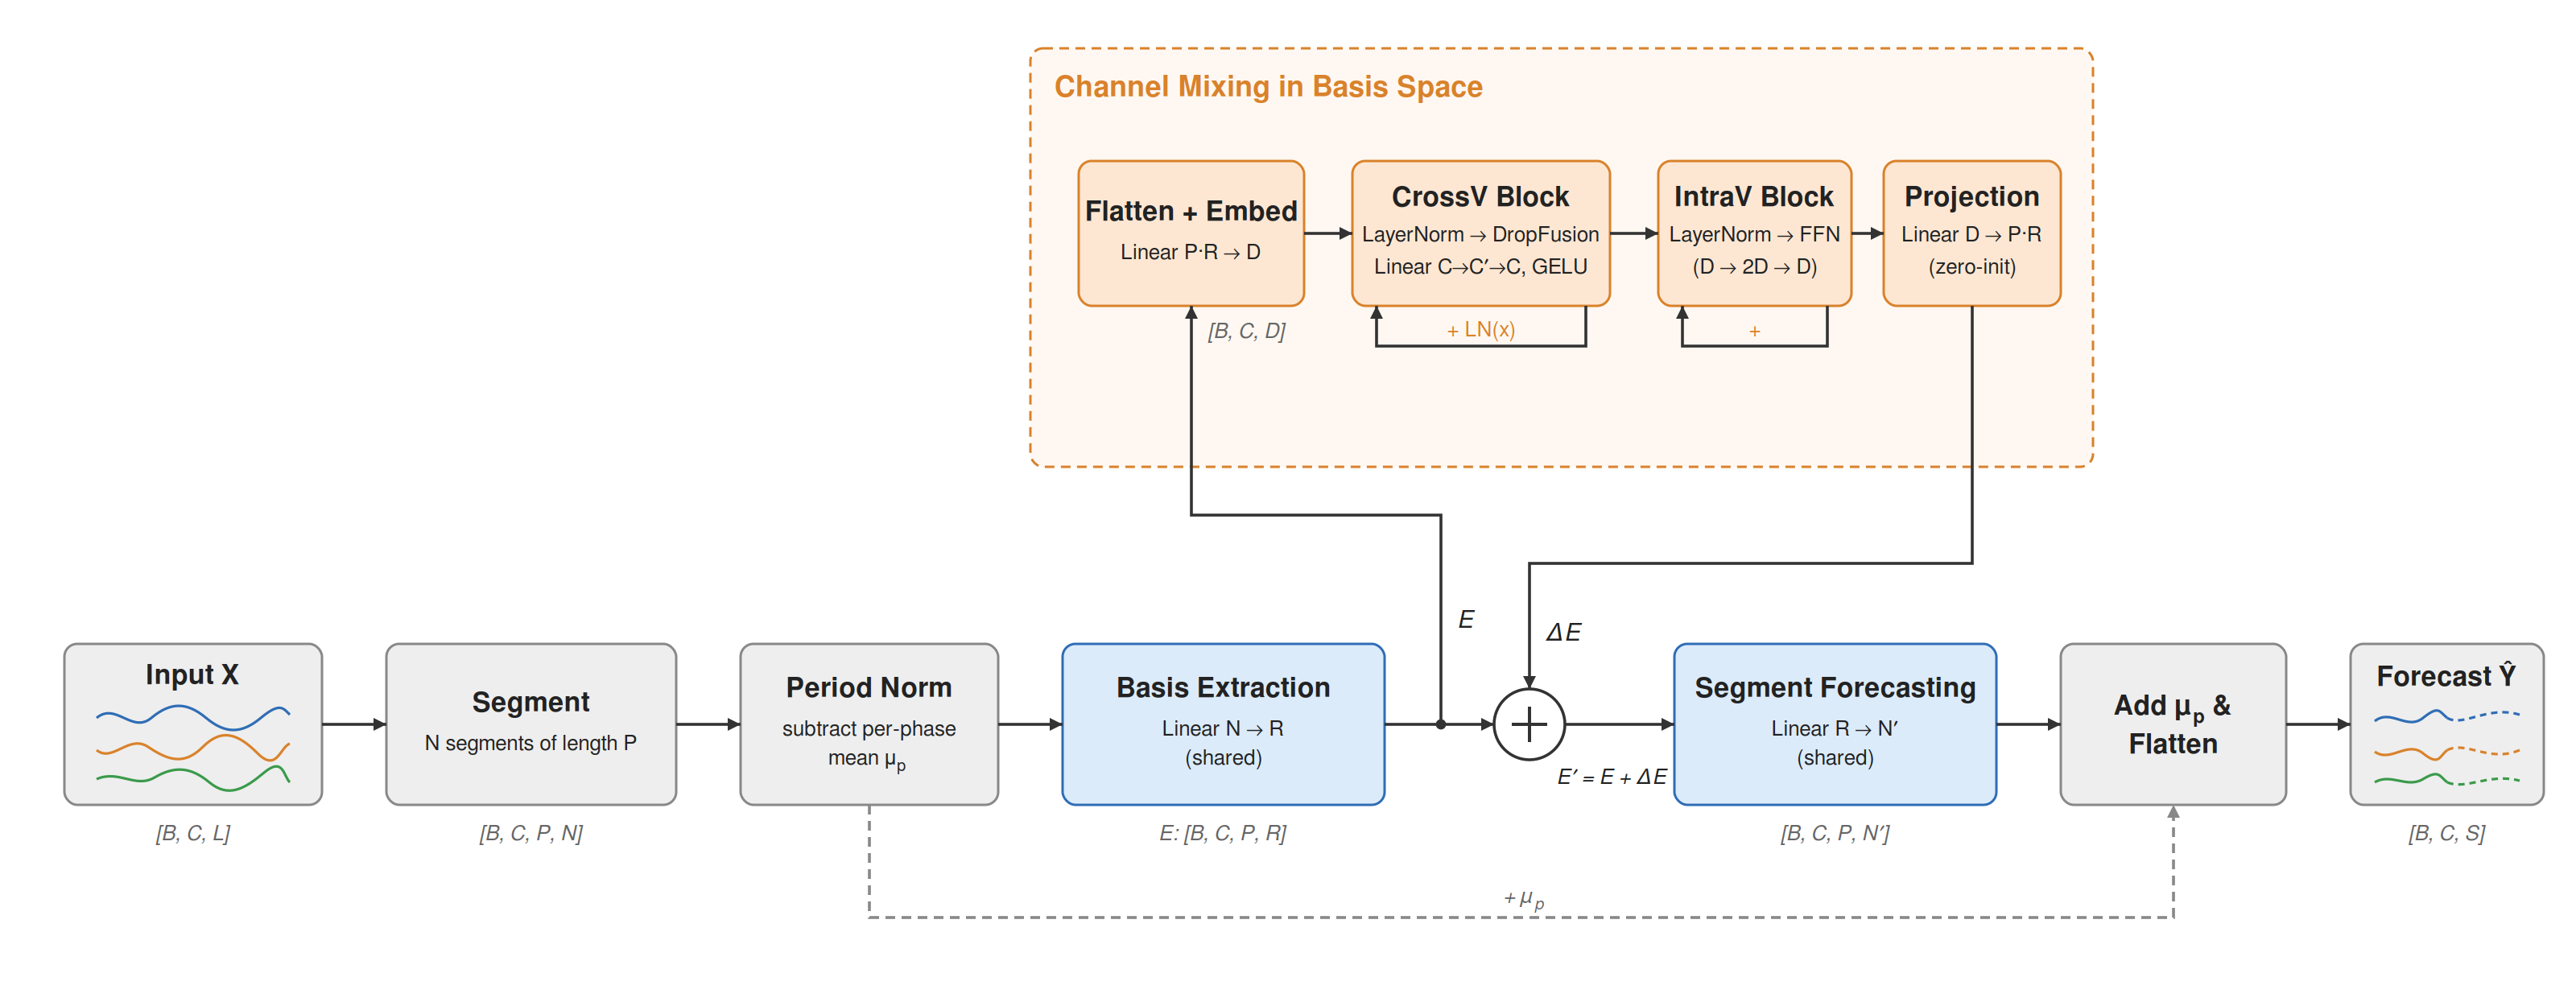
\includegraphics[width=1\linewidth]{dytimebase_architecture.png}

\end{frame}

\begin{frame}{Điều chỉnh và Tối ưu hóa Trọng số}
    \begin{itemize}
        \item Trọng số được cập nhật ngược hướng gradient của hàm mục tiêu $\mathcal{L}$:
        \[ W_{k+1} = W_k - \alpha \frac{\partial \mathcal{L}}{\partial W_k}, \qquad
           b_{k+1} = b_k - \alpha \frac{\partial \mathcal{L}}{\partial b_k} \]

        \item \textbf{Hai tốc độ học:} $\alpha=\alpha_B$ cho $\mathbf{W}_B,\mathbf{b}_B,\mathbf{W}_F,\mathbf{b}_F$,
              $\alpha=\alpha_M$ cho nhánh trộn biến.

        \item \textbf{Tốc độ học} theo epoch $e$: giữ nguyên 4 epoch đầu, sau đó nhân $0.8$ mỗi epoch:
        $\alpha^{(e)} = \alpha$ nếu $e\le 4$, \ $\alpha^{(e)} = \alpha\cdot 0.8^{\,e-4}$ nếu $e>4$.
    \end{itemize}
\end{frame}

\begin{frame}{Vì sao DyBAS-Net nhẹ: Độ phức tạp tính toán}
    \small
    Số phép nhân--cộng (MACs) cho một mẫu:
    \begin{itemize}
        \item \textbf{Xương sống} (trích xuất cơ sở, dự báo theo đoạn): \
        $\text{MACs}_{B} = C\cdot P\cdot R\cdot(N+N')$
        \item \textbf{Nhánh trộn biến:}
        $$\text{MACs}_{M} = \underbrace{2\,C\,PR\,D}_{\text{mã hóa, chiếu ngược}}
          + \underbrace{2\,D\,C\,C'}_{\text{CrossVBlock}} + \underbrace{2\,C\,D\,D_{ff}}_{\text{IntraVBlock}}$$
        \item Không có số hạng nào tỉ lệ với $L\cdot S$; nhánh trộn biến không phụ thuộc $L$ và $S$.
    \end{itemize}

    \begin{block}{Ví dụ Electricity: $C=321$, $L=S=720$, $P=24$, $R=6$, $D=64$}
    $\text{MACs}_B\approx 2.8$M, $\text{MACs}_M\approx 21.0$M, tổng $\approx 23.8$M. \\
    So sánh: DLinear $2CLS\approx 333$M; DyTimeNet $\approx 212$M.
    \end{block}
\end{frame}

%=====================================================================
\section{Thực nghiệm và kết quả}
\subsection{Thiết lập thực nghiệm}

\begin{frame}{Mô tả dữ liệu thực nghiệm}
\begin{center}
\resizebox{\textwidth}{!}{%
\begin{tabular}{@{}lccccc@{}}
\toprule
Dataset & Số biến $C$ & Tần suất & Số bước dùng & Chia Train/Val/Test & Số cửa sổ ($L=720$, $S=96$)\\
\midrule
ETTh1, ETTh2 & 7 & 1 giờ & 14\,400 & 12/4/4 tháng & 7\,825 / 2\,785 / 2\,785\\
ETTm1, ETTm2 & 7 & 15 phút & 57\,600 & 12/4/4 tháng & 33\,745 / 11\,425 / 11\,425\\
Weather & 21 & 10 phút & 52\,696 & 7 : 1 : 2 & 36\,072 / 5\,174 / 10\,445\\
\bottomrule
\end{tabular}}
\end{center}

\begin{itemize}
    \item \textbf{ETT}: nhiệt độ dầu và 6 chỉ số phụ tải của máy biến áp điện.
    \item \textbf{Weather}: 21 chỉ số khí tượng (nhiệt độ, độ ẩm, áp suất, gió\dots), có quan hệ vật lý giữa các biến.
    \item \textbf{Tiền xử lý:} chuẩn hóa Z-score theo từng biến (chỉ tính trên tập train); cửa sổ trượt $L=720$,
          $S\in\{96,192,336,720\}$; đánh giá trên \emph{mọi} cửa sổ của tập test.
\end{itemize}
\end{frame}

\begin{frame}{Siêu tham số của DyBAS-Net}
\begin{center}
\small
\resizebox{\textwidth}{!}{%
\begin{tabular}{lllcccc}
\toprule
 & \multicolumn{3}{c}{Xương sống (theo $S=96/192/336/720$)} & \multicolumn{3}{c}{Nhánh trộn kênh}\\
\cmidrule(lr){2-4}\cmidrule(l){5-7}
Dataset & $P$ & $R$ & Riêng kênh & $D$ & $p_1$ & $p_2$\\
\midrule
ETTh1 & 24/24/24/24 & 6/6/6/6 & không & 64 & 0.1 & 0.1\\
ETTh2 & 24/24/24/24 & 6/4/6/6 & không & 64 & 0.6 & 0.6\\
ETTm1 & 4/4/4/6 & 18/20/20/20 & không & 64 & 0.1 & 0.2\\
ETTm2 & 4/4/4/6 & 20/20/20/20 & không & 32 & 0.1 & 0.1\\
Weather & 4/4/4/4 & 6/6/6/6 & có & 64 & 0.1 & 0.1\\
\bottomrule
\end{tabular}}

\end{center}
\end{frame}

\begin{frame}{Các mô hình so sánh}
\begin{itemize}
    \item \textbf{TimeBase$^{*}$}: TimeBase cài đặt lại theo mã nguồn chính thức (đầu ra lệch $<3\cdot10^{-7}$ so với bản
          gốc khi cùng trọng số), chạy \emph{cùng quy trình} với DyBAS-Net. Hai mô hình chỉ khác nhau ở nhánh trộn biến.

    \vspace{0.15cm}
    \item \textbf{Số liệu công bố} ($L=720$, Table 10 của TimeBase \cite{Huang2025TimeBase}):
    \begin{itemize}
        \item Tuyến tính nhẹ: TimeBase$^{\dagger}$, SparseTSF \cite{Lin2024SparseTSF}, FITS \cite{Xu2024FITS},
              DLinear \cite{Zeng2023DLinear}.
        \item MLP, Transformer, CNN: TimeMixer \cite{Wang2024TimeMixer}, iTransformer \cite{Liu2024iTransformer},
              PatchTST \cite{Nie2023PatchTST}, TimesNet \cite{Wu2023TimesNet}, FEDformer \cite{Zhou2022FEDformer},
              Autoformer \cite{Wu2021Autoformer}, Informer \cite{Zhou2021Informer}.
    \end{itemize}

    \vspace{0.15cm}
    \item Các mô hình lớn không được huấn luyện lại vì chi phí trên CPU quá cao (một epoch của PatchTST ở cấu hình
          Electricity mất khoảng 23 giờ).
\end{itemize}
\end{frame}

\begin{frame}{Chỉ số đánh giá}
\begin{itemize}
    \item \textbf{Độ chính xác:} MSE và MAE trên thang Z-score, lấy trung bình trên mọi cửa sổ test, mọi bước, mọi biến:
    $$\text{MSE} = \frac{1}{n}\sum_{i=1}^{n}(y_i-\hat{y}_i)^2, \qquad \text{MAE} = \frac{1}{n}\sum_{i=1}^{n}|y_i-\hat{y}_i|$$

    \item \textbf{Hiệu năng} (theo TimeBase), cấu hình Electricity ($C=321$, $L=S=720$):
    \begin{itemize}
        \item \textbf{Params}: số tham số; \textbf{MACs}: số phép nhân--cộng cho một mẫu.
        \item \textbf{Max Mem}: bộ nhớ đỉnh khi huấn luyện, lô 12 mẫu (RAM, vì không có GPU).
        \item \textbf{Epoch Time}: thời gian một epoch huấn luyện; \textbf{Infer Time}: dự báo một mẫu trên CPU.
    \end{itemize}

    \item Đo \emph{tất cả mô hình trên cùng máy}, dựng từ mã nguồn chính thức (Time-Series-Library \cite{Wang2024TSLib},
          kho mã của PatchTST và FITS).
\end{itemize}
\end{frame}

\subsection{Kết quả độ chính xác}

\begin{frame}{Kết quả: MSE / MAE trung bình trên 4 độ dài dự báo}
\scriptsize
\resizebox{\textwidth}{!}{%
\begin{tabular}{lcccccccccc}
\toprule
\multirow{2}{*}{Mô hình} & \multicolumn{2}{c}{ETTh1} & \multicolumn{2}{c}{ETTh2} & \multicolumn{2}{c}{ETTm1} & \multicolumn{2}{c}{ETTm2} & \multicolumn{2}{c}{Weather}\\
\cmidrule(lr){2-3}\cmidrule(lr){4-5}\cmidrule(lr){6-7}\cmidrule(lr){8-9}\cmidrule(lr){10-11}
 & MSE & MAE & MSE & MAE & MSE & MAE & MSE & MAE & MSE & MAE\\
\midrule
\textbf{DyBAS-Net} & \underline{0.403} & 0.421 & 0.358 & 0.406 & \textbf{0.351} & 0.386 & 0.263 & 0.330 & \underline{0.221} & 0.277\\
TimeBase$^{*}$ & 0.411 & 0.420 & 0.363 & 0.410 & 0.367 & 0.391 & 0.254 & \underline{0.317} & \textbf{0.219} & 0.265\\
TimeBase$^{\dagger}$ & \textbf{0.396} & \textbf{0.414} & 0.347 & 0.397 & 0.356 & \textbf{0.381} & \textbf{0.251} & \textbf{0.314} & \textbf{0.219} & \textbf{0.263}\\
\midrule
SparseTSF & 0.407 & \underline{0.419} & \underline{0.344} & \underline{0.387} & 0.362 & 0.384 & 0.253 & \underline{0.317} & 0.244 & 0.285\\
TimeMixer & 0.454 & 0.474 & 0.379 & 0.426 & 0.381 & 0.414 & 0.283 & 0.347 & 0.238 & 0.281\\
FITS & 0.417 & 0.430 & \textbf{0.334} & \textbf{0.382} & 0.359 & \underline{0.382} & \underline{0.252} & \textbf{0.314} & 0.244 & 0.286\\
iTransformer & 0.454 & 0.467 & 0.392 & 0.422 & 0.370 & 0.401 & 0.278 & 0.338 & 0.233 & 0.273\\
DLinear & 0.437 & 0.448 & 0.479 & 0.471 & 0.361 & 0.383 & 0.271 & 0.337 & 0.242 & 0.299\\
PatchTST & 0.420 & 0.440 & \underline{0.344} & 0.391 & \underline{0.355} & 0.385 & \textbf{0.251} & 0.319 & 0.224 & \underline{0.264}\\
TimesNet & 0.505 & 0.499 & 0.433 & 0.455 & 0.408 & 0.425 & 0.299 & 0.353 & 0.254 & 0.293\\
FEDformer & 0.523 & 0.523 & 0.429 & 0.470 & 0.439 & 0.466 & 0.409 & 0.462 & 0.355 & 0.391\\
Autoformer & 0.727 & 0.641 & 1.086 & 0.801 & 0.564 & 0.522 & 0.431 & 0.463 & 0.446 & 0.457\\
Informer & 1.445 & 0.929 & 5.486 & 1.891 & 1.138 & 0.818 & 3.594 & 1.473 & 0.567 & 0.513\\
\bottomrule
\end{tabular}}


\vspace{0.1cm}
$^{*}$ TimeBase đo trên máy này, cùng quy trình với DyBAS-Net, trung bình 3 seed. Các mô hình dưới vạch kẻ: số công bố
trong \cite{Huang2025TimeBase}, cùng $L=720$; trung bình tính từ kết quả theo từng $S$ (Table 10).
\textcolor{red}{\textbf{Đỏ}}: tốt nhất; \textcolor{blue}{xanh}: thứ hai.
\end{frame}

\begin{frame}{Nhận xét kết quả độ chính xác}
\begin{itemize}
    \item \textbf{ETTh1, ETTm1:} DyBAS-Net có MSE \textbf{thấp nhất} trong bảng (0.403 và 0.351), tốt hơn SparseTSF
          (0.407) trên ETTh1 và PatchTST (0.355) trên ETTm1.
    \item \textbf{Weather:} DyBAS-Net đứng \textbf{thứ hai} về MSE (0.221), chỉ sau TimeBase$^{*}$ (0.219); tốt hơn
          PatchTST, SparseTSF, FITS và mọi mô hình Transformer.
    \item \textbf{ETTh2, ETTm2:} DyBAS-Net (0.358 và 0.263) kém nhóm tuyến tính mạnh (FITS, SparseTSF, TimeBase$^{*}$) và
          PatchTST.
    \item \textbf{MAE:} cải thiện ít hơn MSE; trên phần lớn bộ dữ liệu, MAE của DyBAS-Net không tốt hơn TimeBase$^{*}$.
\end{itemize}
\end{frame}

\begin{frame}{Kết quả theo độ dài dự báo $S$ (MSE): ETTh1, ETTh2}
\scriptsize
\resizebox{\textwidth}{!}{%
\begin{tabular}{llccccccccc}
\toprule
Dataset & $S$ & \textbf{DyBAS-Net} & TimeBase$^{*}$ & TimeBase$^{\dagger}$ & SparseTSF & FITS & PatchTST & iTransformer & DLinear & TimeMixer\\
\midrule
\multirow{4}{*}{ETTh1} & 96 & \textbf{0.347} & 0.358 & \underline{0.349} & 0.362 & 0.380 & 0.377 & 0.389 & 0.378 & 0.410\\
 & 192 & \underline{0.388} & 0.396 & \textbf{0.387} & 0.404 & 0.415 & 0.413 & 0.424 & 0.415 & 0.448\\
 & 336 & \underline{0.420} & 0.423 & \textbf{0.408} & 0.435 & 0.439 & 0.436 & 0.456 & 0.449 & 0.482\\
 & 720 & 0.456 & 0.466 & 0.439 & \textbf{0.426} & \underline{0.433} & 0.455 & 0.545 & 0.507 & 0.475\\
\midrule
\multirow{4}{*}{ETTh2} & 96 & 0.286 & 0.295 & 0.292 & 0.294 & \textbf{0.271} & \underline{0.276} & 0.305 & 0.294 & 0.315\\
 & 192 & 0.347 & 0.352 & \underline{0.339} & 0.340 & \textbf{0.332} & 0.342 & 0.405 & 0.412 & 0.383\\
 & 336 & 0.378 & 0.390 & \underline{0.358} & 0.360 & \textbf{0.355} & 0.364 & 0.411 & 0.471 & 0.385\\
 & 720 & 0.421 & 0.413 & 0.400 & \underline{0.383} & \textbf{0.378} & 0.395 & 0.448 & 0.740 & 0.432\\
\bottomrule
\end{tabular}}


\vspace{0.1cm}
\textcolor{red}{\textbf{Đỏ}}: tốt nhất; \textcolor{blue}{xanh}: thứ hai (xếp hạng trên cả 13 mô hình). Không hiển thị TimesNet, FEDformer, Autoformer, Informer
(DyBAS-Net tốt hơn ở mọi ô).
\end{frame}

\begin{frame}{Kết quả theo độ dài dự báo $S$ (MSE): ETTm1, ETTm2}
\scriptsize
\resizebox{\textwidth}{!}{%
\begin{tabular}{llccccccccc}
\toprule
Dataset & $S$ & \textbf{DyBAS-Net} & TimeBase$^{*}$ & TimeBase$^{\dagger}$ & SparseTSF & FITS & PatchTST & iTransformer & DLinear & TimeMixer\\
\midrule
\multirow{4}{*}{ETTm1} & 96 & \textcolor{red}{\textbf{0.296}} & 0.318 & 0.311 & 0.314 & 0.313 & \textcolor{blue}{0.298} & 0.315 & 0.314 & 0.332\\
 & 192 & \textcolor{red}{\textbf{0.328}} & 0.363 & 0.338 & 0.348 & 0.339 & \textcolor{blue}{0.335} & 0.349 & 0.347 & 0.355\\
 & 336 & \textcolor{red}{\textbf{0.364}} & 0.372 & \textcolor{red}{\textbf{0.364}} & 0.368 & 0.367 & \textcolor{blue}{0.366} & 0.381 & 0.367 & 0.386\\
 & 720 & 0.416 & 0.418 & \textcolor{red}{\textbf{0.413}} & 0.419 & 0.417 & 0.420 & 0.437 & \textcolor{blue}{0.415} & 0.452\\
\midrule
\multirow{4}{*}{ETTm2} & 96 & 0.167 & 0.166 & \textcolor{red}{\textbf{0.162}} & 0.167 & 0.166 & 0.165 & 0.179 & \textcolor{blue}{0.163} & 0.192\\
 & 192 & 0.237 & \textcolor{red}{\textbf{0.218}} & \textcolor{red}{\textbf{0.218}} & \textcolor{blue}{0.219} & \textcolor{red}{\textbf{0.218}} & \textcolor{blue}{0.219} & 0.239 & 0.223 & 0.253\\
 & 336 & 0.284 & 0.277 & \textcolor{blue}{0.270} & 0.271 & 0.271 & \textcolor{red}{\textbf{0.268}} & 0.309 & 0.291 & 0.307\\
 & 720 & 0.366 & 0.355 & \textcolor{red}{\textbf{0.352}} & \textcolor{blue}{0.353} & \textcolor{red}{\textbf{0.352}} & \textcolor{red}{\textbf{0.352}} & 0.387 & 0.407 & 0.380\\
\bottomrule
\end{tabular}}


\vspace{0.1cm}
\textcolor{red}{\textbf{Đỏ}}: tốt nhất; \textcolor{blue}{xanh}: thứ hai (xếp hạng trên cả 13 mô hình).
\end{frame}

\begin{frame}{Kết quả theo độ dài dự báo $S$ (MSE): Weather}
\scriptsize
\resizebox{\textwidth}{!}{%
\begin{tabular}{llcccccccc}
\toprule
Dataset & $S$ & \textbf{DyBAS-Net} & TimeBase & SparseTSF & FITS & PatchTST & iTransformer & DLinear & TimeMixer\\
\midrule
\multirow{4}{*}{Weather} & 96 & \textcolor{red}{\textbf{0.143}} & \textcolor{blue}{0.144} & 0.174 & 0.176 & 0.149 & 0.159 & 0.174 & 0.163\\
 & 192 & \textcolor{red}{\textbf{0.187}} & \textcolor{red}{\textbf{0.187}} & 0.216 & 0.216 & \textcolor{blue}{0.193} & 0.203 & 0.215 & 0.201\\
 & 336 & \textcolor{blue}{0.240} & \textcolor{red}{\textbf{0.238}} & 0.260 & 0.261 & \textcolor{blue}{0.240} & 0.253 & 0.262 & 0.258\\
 & 720 & 0.314 & \textcolor{red}{\textbf{0.309}} & 0.325 & 0.325 & \textcolor{blue}{0.312} & 0.317 & 0.319 & 0.329\\
\bottomrule
\end{tabular}}


\vspace{0.1cm}
\textcolor{red}{\textbf{Đỏ}}: tốt nhất; \textcolor{blue}{xanh}: thứ hai (xếp hạng trên cả 13 mô hình).

\vspace{0.2cm}
\small
\begin{itemize}
    \item Weather có nhiều biến nhất (21) và quan hệ vật lý giữa các biến rõ nhất.
    \item DyBAS-Net tốt nhất ở $S=96$ (0.143); ở $S=192$ ngang TimeBase$^{*}$ (0.187); ở $S=336$ và $S=720$ kém TimeBase
          một chút.
\end{itemize}
\end{frame}

\begin{frame}{DyBAS-Net đối đầu từng mô hình}
\scriptsize
\resizebox{\textwidth}{!}{%
\begin{tabular}{lcccll}
\toprule
Đối thủ & Thắng & Hòa & Thua & DyBAS-Net tốt hơn (MSE TB) & DyBAS-Net kém hơn (MSE TB)\\
\midrule
TimeBase & 12 & 2 & 6 & ETTh1, ETTh2, ETTm1 & ETTm2, Weather\\
CycleNet-L & 12 & 0 & 8 & ETTh1, ETTm1, Weather & ETTh2, ETTm2\\
CycleNet-M & 17 & 0 & 3 & ETTh1, ETTh2, ETTm1, Weather & ETTm2\\
TQNet & 16 & 0 & 4 & ETTh1, ETTh2, ETTm1, Weather & ETTm2\\
SparseTSF & 13 & 0 & 7 & ETTh1, ETTm1, Weather & ETTh2, ETTm2\\
TimeMixer & 19 & 0 & 1 & ETTh1, ETTh2, ETTm1, ETTm2, Weather & --\\
FITS & 11 & 1 & 8 & ETTh1, ETTm1, Weather & ETTh2, ETTm2\\
iTransformer & 20 & 0 & 0 & ETTh1, ETTh2, ETTm1, ETTm2, Weather & --\\
DLinear & 17 & 0 & 3 & ETTh1, ETTh2, ETTm1, ETTm2, Weather & --\\
PatchTST & 9 & 2 & 9 & ETTh1, ETTm1, Weather & ETTh2, ETTm2\\
TimesNet & 20 & 0 & 0 & ETTh1, ETTh2, ETTm1, ETTm2, Weather & --\\
FEDformer & 20 & 0 & 0 & ETTh1, ETTh2, ETTm1, ETTm2, Weather & --\\
Autoformer & 20 & 0 & 0 & ETTh1, ETTh2, ETTm1, ETTm2, Weather & --\\
Informer & 20 & 0 & 0 & ETTh1, ETTh2, ETTm1, ETTm2, Weather & --\\
\bottomrule
\end{tabular}}


\vspace{0.15cm}
\small
Đếm trên 20 ô (5 bộ dữ liệu $\times$ 4 độ dài dự báo) theo MSE, làm tròn 3 chữ số.
\begin{itemize}
    \item \textbf{Hơn hẳn:} TimeMixer, iTransformer, TimesNet, FEDformer, Autoformer, Informer (20/20) và DLinear (17/20).
    \item \textbf{Ngang ngửa:} SparseTSF, FITS, PatchTST (thắng trên ETTh1, ETTm1, Weather; thua trên ETTh2, ETTm2).
    \item \textbf{Kém hơn:} số công bố của TimeBase (thắng 5/20).
\end{itemize}
\end{frame}

\begin{frame}{So sánh với TimeBase trong cùng quy trình}
\small
Thay đổi MSE của DyBAS-Net so với TimeBase$^{*}$ (âm là tốt hơn). Hai mô hình dùng cùng xương sống, cùng siêu tham số
xương sống, cùng 3 seed, chỉ khác ở nhánh trộn biến:

\vspace{0.15cm}
\scriptsize
\resizebox{0.75\textwidth}{!}{%
\begin{tabular}{lccccc}
\toprule
Dataset & $S=96$ & $S=192$ & $S=336$ & $S=720$ & Trung bình\\
\midrule
ETTh1 & \textcolor{ForestGreen}{$-2.8\%$} & \textcolor{ForestGreen}{$-2.0\%$} & \textcolor{ForestGreen}{$-0.5\%$} & \textcolor{ForestGreen}{$-2.1\%$} & \textcolor{ForestGreen}{$-1.8\%$}\\
ETTh2 & \textcolor{ForestGreen}{$-6.0\%$} & \textcolor{ForestGreen}{$-3.1\%$} & \textcolor{ForestGreen}{$-1.1\%$} & \textcolor{mqred}{$+0.4\%$} & \textcolor{ForestGreen}{$-2.1\%$}\\
ETTm1 & \textcolor{ForestGreen}{$-6.8\%$} & \textcolor{ForestGreen}{$-9.6\%$} & \textcolor{ForestGreen}{$-2.0\%$} & \textcolor{ForestGreen}{$-0.5\%$} & \textcolor{ForestGreen}{$-4.5\%$}\\
ETTm2 & \textcolor{ForestGreen}{$-0.1\%$} & \textcolor{mqred}{$+7.3\%$} & \textcolor{mqred}{$+4.3\%$} & \textcolor{mqred}{$+3.8\%$} & \textcolor{mqred}{$+4.0\%$}\\
Weather & \textcolor{ForestGreen}{$-0.4\%$} & \textcolor{mqred}{$+0.1\%$} & \textcolor{mqred}{$+0.9\%$} & \textcolor{mqred}{$+1.6\%$} & \textcolor{mqred}{$+0.8\%$}\\
\bottomrule
\end{tabular}}


\vspace{0.15cm}
\small
\begin{itemize}
    \item Nhánh trộn biến \textbf{cải thiện 3/5 bộ dữ liệu}: ETTh1 ($-1.8\%$), ETTh2 ($-1.3\%$), ETTm1 ($-4.5\%$).
    \item Cải thiện lớn nhất ở dự báo ngắn: ETTm1 với $S=192$ giảm $9.6\%$.
    \item \textbf{ETTm2} kém hơn ($+3.7\%$): các lần chạy thường dừng sau 6--7 epoch, nhánh phi tuyến quá khớp trên chuỗi
          tương đối trơn.
\end{itemize}
\end{frame}

\subsection{Kết quả hiệu năng}

\begin{frame}{Hiệu năng tính toán trên cùng một thiết bị}
\scriptsize
Electricity ($C=321$), $L=S=720$. Max Mem: đỉnh RAM khi huấn luyện, lô 12 mẫu. Epoch Time: thời gian một bước huấn luyện
(lô 12) $\times$ 1\,414 bước. Infer Time: dự báo 1 mẫu, 8 luồng. Sắp xếp theo Infer Time.

\vspace{0.1cm}
\resizebox{\textwidth}{!}{%
\begin{tabular}{lrrrrrr}
\toprule
Mô hình & Params & MACs & Max Mem (MB) & Epoch Time (s) & Infer Time (ms) & So với DyBAS-Net\\
\midrule
TimeBase & 0.40K & 2.77M & 117 & 20 & 0.34 & 0.52$\times$\\
\textbf{DyBAS-Net} & 190.51K & 23.81M & 147 & 38 & 0.66 & 1.00$\times$\\
SparseTSF & 0.93K & 12.71M & 276 & 56 & 0.76 & 1.15$\times$\\
FITS & 133.64K & 42.73M & 210 & 78 & 1.70 & 2.59$\times$\\
DLinear & 1.04M & 332.81M & 150 & 55 & 1.93 & 2.94$\times$\\
DyTimeNet & 785.14K & 211.80M & 285 & 131 & 2.14 & 3.25$\times$\\
iTransformer & 5.47M & 2.10G & 997 & 695 & 10.66 & 16.23$\times$\\
Informer & 12.45M & 7.91G & 2\,052 & 2\,926 & 66.16 & 100.66$\times$\\
Autoformer & 12.14M & 8.97G & 5\,057 & 5\,302 & 83.39 & 126.88$\times$\\
FEDformer & 18.44M & 8.99G & 3\,289 & 5\,367 & 135.93 & 206.81$\times$\\
TimeMixer & 5.58M & 29.97G & $>$11\,264$^{\ddagger}$ & 16\,716 & 247.46 & 376.51$\times$\\
PatchTST & 8.69M & 16.08G & 10\,346 & 82\,400 & 285.51 & 434.40$\times$\\
TimesNet & 151.32M & 1081.75G & 4\,078 & 170\,983 & 3\,449.01 & 5\,247.64$\times$\\
\bottomrule
\end{tabular}}


\vspace{0.05cm}
{\tiny $^{\ddagger}$ Vượt ngưỡng 11 GB RAM ở lô 12; Epoch Time của mô hình này đo ở lô 4.}
\end{frame}

\begin{frame}{Nhận xét hiệu năng}
\begin{itemize}
    \item DyBAS-Net \textbf{nhanh thứ hai trong 13 mô hình} khi suy luận (0.66 ms một mẫu), chỉ sau TimeBase (0.34 ms).
    \item Nhanh hơn SparseTSF (0.76 ms), FITS (1.70 ms), DLinear (1.93 ms).
    \item So với Transformer: nhanh hơn iTransformer $\sim$16 lần, TimeMixer $\sim$377 lần, PatchTST $\sim$434 lần.
    \item Huấn luyện nhẹ: 38 s một epoch, 147 MB bộ nhớ (PatchTST: hơn 10 GB, khoảng 23 giờ một epoch).
    \item So với DyTimeNet (Đồ án I): ít hơn $\sim$4.1 lần tham số, $\sim$8.9 lần MACs, suy luận nhanh hơn $\sim$3.2 lần.
\end{itemize}

\begin{block}{Nguyên nhân}
Biến đổi theo trục thời gian chạy trên $N$, $R$, $P$ (vài chục) thay vì $L$, $S$ (hàng trăm); không có attention.
\end{block}
\end{frame}

\subsection{Nghiên cứu loại bỏ}

\begin{frame}{Nghiên cứu loại bỏ (Ablation study)}
\small
MSE trung bình trên 4 độ dài dự báo và 3 seed; mỗi biến thể chỉ bỏ một khối, giữ nguyên mọi siêu tham số khác.

\vspace{0.15cm}
\scriptsize
\resizebox{\textwidth}{!}{%
\begin{tabular}{lcccccc}
\toprule
Biến thể & ETTh1 & ETTh2 & ETTm1 & ETTm2 & Weather & Trung bình\\
\midrule
\textbf{DyBAS-Net (đầy đủ)} & 0.4030 & \textcolor{blue}{0.3580} & \textcolor{red}{\textbf{0.3509}} & 0.2634 & 0.2211 & \textcolor{blue}{0.3193}\\
\quad bỏ CrossVBlock & 0.4028 & 0.3595 & 0.3554 & \textcolor{blue}{0.2615} & 0.2226 & 0.3204\\
\quad bỏ IntraVBlock & \textcolor{blue}{0.4004} & 0.3668 & \textcolor{blue}{0.3524} & 0.2661 & \textcolor{red}{\textbf{0.2186}} & 0.3209\\
\quad bỏ cả nhánh ($=$ TimeBase$^{*}$) & 0.4105 & 0.3627 & 0.3674 & \textcolor{red}{\textbf{0.2539}} & \textcolor{blue}{0.2195} & 0.3228\\
\midrule
đầy đủ, $\alpha_M = 2\cdot10^{-3}$ & \textcolor{red}{\textbf{0.3992}} & \textcolor{red}{\textbf{0.3569}} & 0.3554 & 0.2627 & 0.2203 & \textcolor{red}{\textbf{0.3189}}\\
\bottomrule
\end{tabular}}


\vspace{0.1cm}
\textcolor{red}{\textbf{Đỏ}}: tốt nhất; \textcolor{blue}{xanh}: thứ hai (mỗi cột).

\vspace{0.2cm}
\small
Các biến thể ``bỏ khối'' chỉ dùng để kiểm chứng; mô hình đề xuất là DyBAS-Net đầy đủ.
\end{frame}

\begin{frame}{Nhận xét nghiên cứu loại bỏ}
\begin{itemize}
    \item Tính trung bình, \textbf{bản đầy đủ tốt hơn mọi bản đã bỏ khối}: bỏ CrossVBlock (0.3204), bỏ IntraVBlock (0.3209),
          bỏ cả nhánh (0.3228) so với 0.3193.
    \item \textbf{Weather} (21 biến): bỏ CrossVBlock cho kết quả kém nhất (0.2226); chỉ giữ CrossVBlock cho kết quả tốt nhất
          (0.2186), tốt hơn TimeBase$^{*}$. Trộn biến có ích hơn khi có nhiều biến.
    \item Tăng $\alpha_M$ lên $2\cdot10^{-3}$ gần như không đổi (0.3189), nên giữ cấu hình của Đồ án I.
\end{itemize}
\end{frame}

%=====================================================================
\section{Kết luận}

\begin{frame}{Kết luận}
\begin{itemize}
    \item \textbf{Đề xuất DyBAS-Net:} kết hợp dự báo theo đoạn dựa trên thành phần cơ sở (TimeBase) với học phụ thuộc chéo
          có điều chuẩn thưa (CrossVBlock, DropFusion, IntraVBlock của DyTimeNet), đặt trong \emph{không gian cơ sở}.
    \item \textbf{Rất nhẹ:} 23.8M MACs, 0.66 ms một mẫu trên CPU ở cấu hình Electricity; nhanh thứ hai trong 13 mô hình,
          nhanh hơn các mô hình Transformer từ 16 đến hàng nghìn lần.
    \item \textbf{Chính xác cạnh tranh:} tốt nhất trên ETTm1, thứ hai trên ETTh1 và Weather; vượt toàn bộ mô hình
          Transformer và DLinear; ngang ngửa SparseTSF, FITS, PatchTST.
    \item \textbf{Nhánh trộn biến có ích:} so với TimeBase cùng quy trình, giảm MSE trên 3/5 bộ dữ liệu (tới $4.5\%$ trên
          ETTm1); ablation cho thấy cả CrossVBlock và IntraVBlock đều đóng góp.
\end{itemize}
\end{frame}

\begin{frame}{Hạn chế}
\begin{itemize}
    \item \textbf{Chưa vượt số công bố của TimeBase} về độ chính xác; kém các mô hình tuyến tính mạnh trên ETTh2, ETTm2.
    \item \textbf{Quá khớp trên dữ liệu trơn:} trên ETTm2, nhánh phi tuyến làm MSE tăng $3.7\%$ so với TimeBase.
    \item \textbf{Mức cải thiện nhỏ:} các chênh lệch trong ablation ($0.3$--$1.1\%$) cùng cỡ độ lệch chuẩn giữa các seed.
    \item \textbf{Chậm hơn TimeBase} khoảng 2 lần, cái giá của nhánh trộn biến.
    \item \textbf{Phạm vi đánh giá:} số liệu của 10 mô hình lớn là số trích dẫn; hiệu năng đo trên CPU (Max Mem là RAM,
          Epoch Time của mô hình lớn là ước tính từ một bước huấn luyện).
\end{itemize}
\end{frame}

%=====================================================================
\section{Tài liệu tham khảo}
\begin{frame}[allowframebreaks]{Tài liệu tham khảo}
    \renewcommand*{\bibfont}{\tiny}
    \printbibliography[heading=none]
\end{frame}

\end{document}
